\pattern{Pipe and Filter}
\begin{summary}

    A very simple, powerful, and robust architectural style comprised of
    filters, which are used to transform data, and pipes, which pass the data
    between them.

    {\bf Pipe and filter} is most useful for asynchronous systems with many
    data transformations and large processes that can be broken down into
    sub-tasks. The style allows concurrent and modular application of filters
    to subsets of the data. Filters must sometimes be serialized (applied
    one after another) and thus don’t always benefit from concurrency (but
    still benefit from modularity). 
    
    This architectural style also applies to systems where the output of one
    program becomes the input of another program like the UNIX pipe command
    (which is where the name comes from).

\end{summary}

\subsubsection{Implementation}

\begin{description}
    \item[Pipe] Carries and transfers data between components (pumps,
        filters, and sinks). Pipes are directional streams of data, and are
        generally implemented as a type of data buffer which stores data until
        the next filter or sink is available to take the data and process it. A
        pipe can be thought of as a connector between two components.

    \item[Filter] A component of the system which performs some processing to
        the data delivered to it by a pipe. The processed data is output to
        another pipe. A filter can have any amount of input and output pipes.

    \item[Pump] A data source to the overall system. Pumps can be files as well
        as input devices such as keyboards, mice, etc.

    \item[Sink] The ultimate data target (output receiver) of the system.
        Sinks can be files, databases, output devices (screen, speakers), etc.
\end{description}

\comparison{\begin{description}
        \item[Modularity] Components can be pipelined together in many
            different combinations to create novel applications. Each component
            is completely separate for maintenance and development purposes.

        \item[Scalability] Developers can compile and run components in
            parallel since they have defined inputs and outputs with no side
            effects.

        \item[Maintainability] Components do not rely on the implementation of
            each other, so are easy to test. The encapsulation is useful to
            create hierarchy and simplifies the use of this style.

        \item[Maintainabilty] The style creates reusable code due to the
            separation of concerns of each component

    \end{description}
}{\begin{description}
        \item[Flexibility] Pipe-and-filter is not ideal for passing complex
            data structures between the components, because they would need to
            be serialized to a common data type. 

            It is not useful when components need to interact because pipes do
            not allow shared access. If the filters are distributed, the
            usual caveats of distributed computing apply.

    \end{description}
}% END Comparison

\begin{nfps}
\item[Efficiency] Filters work independently to each other, which leads to a
    very efficient workflow as no components depend on others to work.

\item[Scalability] The system can be scaled up or down by simply adding or
    removing filters and different pipes.

\item[Maintainability] As mentioned previously. 
    
\item[Negative Evolvability] The cost and development time of the design might
    be higher than similar designs, as each component is designed individually. 

\item [Negative Resilience] Since one broken filter can defect the entire
    system, if it is the only instance, and the work cannot be rescheduled.

\end{nfps}

\begin{center}
    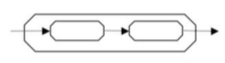
\includegraphics[width=0.4\textwidth]{./pipe-filter}
    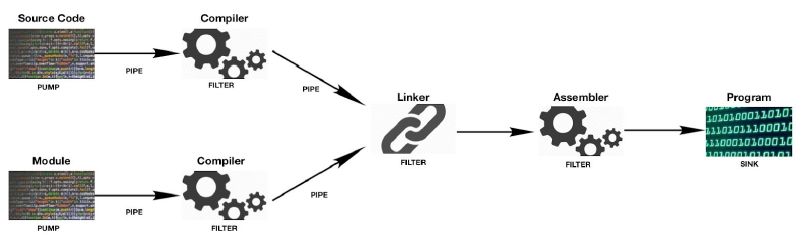
\includegraphics[width=0.4\textwidth]{./pipe-filter2}
\end{center}
